\documentclass[border=8pt]{standalone}

\usepackage{pgfplots}
\pgfplotsset{compat=1.18}

% ----------------------------------------------------------
%  Cornell Palette
% ----------------------------------------------------------
\definecolor{CornellRed}   {RGB}{179, 27,  27}
\definecolor{CornellDark}  {RGB}{ 91,  0,   0}
\definecolor{CornellMid}   {RGB}{140, 20,  20}
\definecolor{CornellAccent}{RGB}{220,170,170}
\definecolor{CornellLight} {RGB}{250,238,238}
\definecolor{CornellGray}  {RGB}{ 84, 88,  90}
\definecolor{LoRABlue}     {RGB}{ 60,100,165}
\definecolor{NumGreen}     {RGB}{ 30,120, 60}
\definecolor{BodyBg}       {RGB}{255,255,255}
\definecolor{TableShade}   {RGB}{253,238,238}

\begin{document}
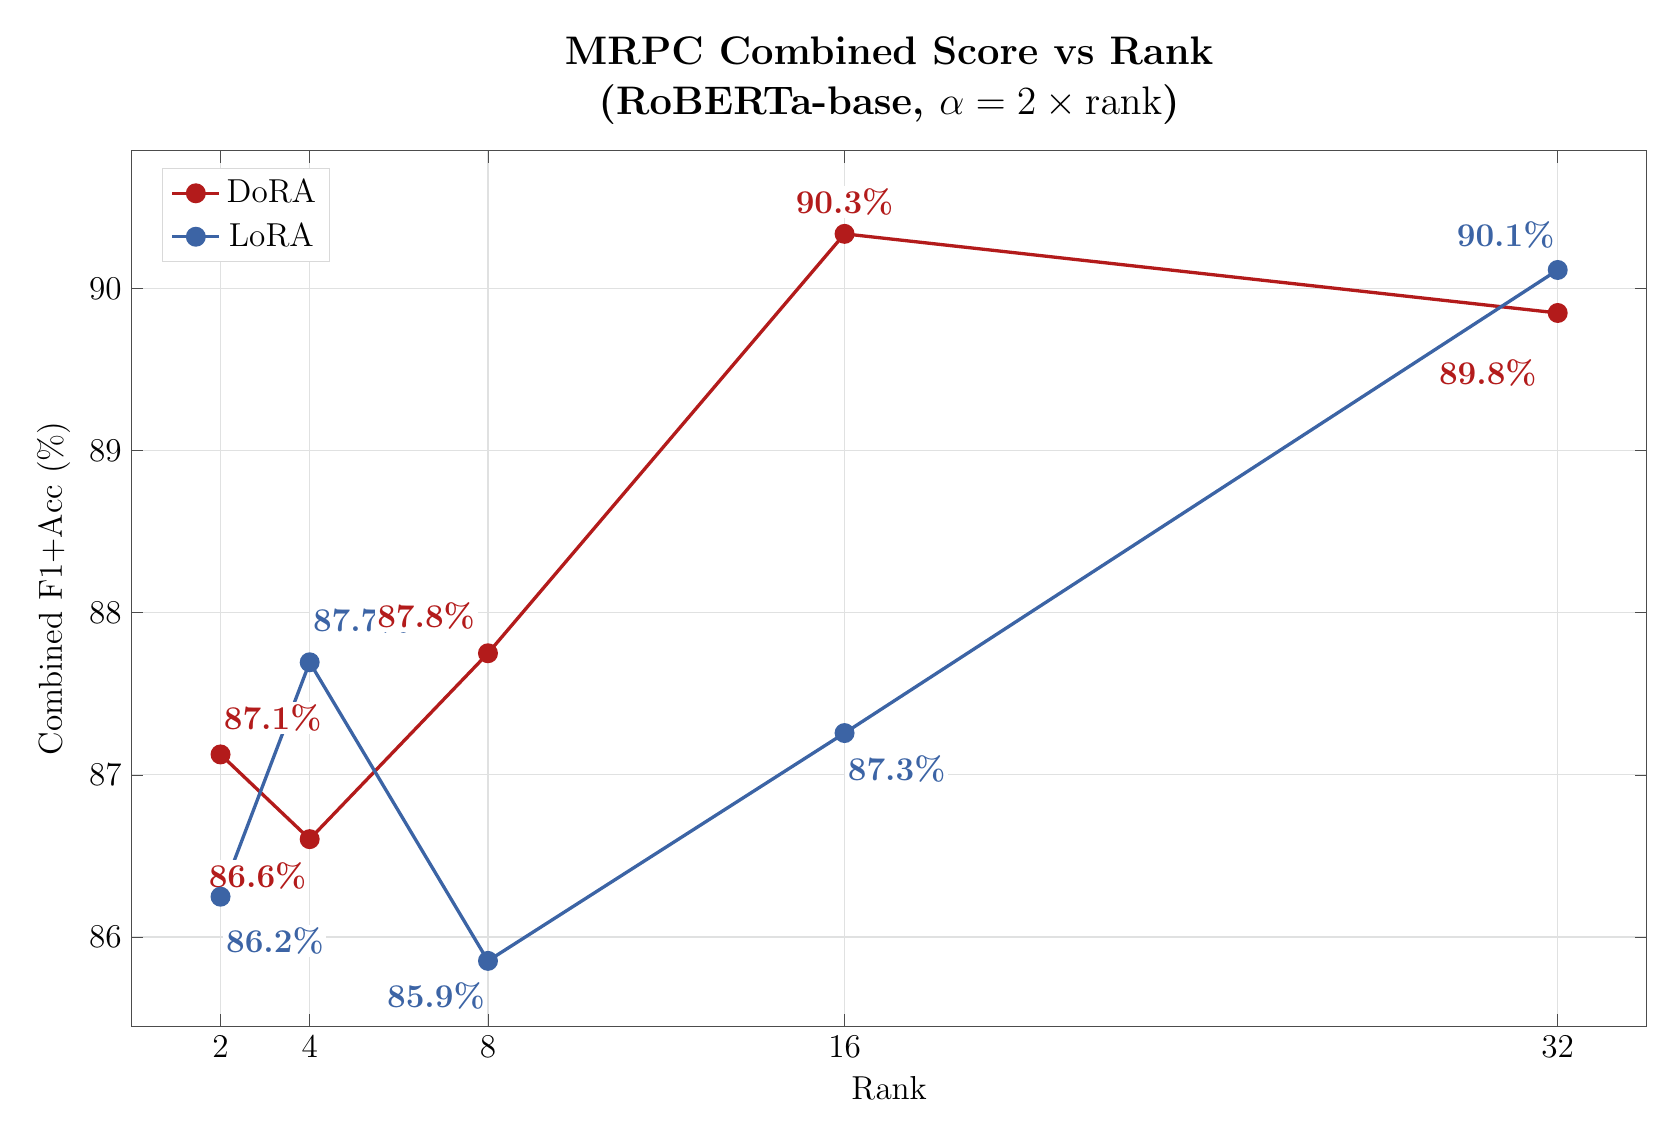
\begin{tikzpicture}
\begin{axis}[
    width=8.2in,
    height=5.0in,
    title={MRPC Combined Score vs Rank\\(RoBERTa-base, $\alpha = 2 \times \mathrm{rank}$)},
    title style={font=\bfseries\Large, align=center},
    xlabel={Rank},
    ylabel={Combined F1+Acc (\%)},
    label style={font=\large},
    tick label style={font=\large},
    xmin=0,
    xmax=34,
    ymin=85.45,
    ymax=90.85,
    xtick={2,4,8,16,32},
    xticklabels={2,4,8,16,32},
    ytick={86,87,88,89,90},
    grid=major,
    major grid style={draw=CornellGray!18},
    axis line style={draw=black!70},
    tick style={draw=black!70},
    legend style={
        at={(0.02,0.98)},
        anchor=north west,
        draw=black!15,
        fill=BodyBg,
        font=\large,
        row sep=2pt
    },
]

\addplot[
    CornellRed,
    very thick,
    mark=*,
    mark size=3.0pt,
] coordinates {
    (2,87.1263)
    (4,86.6037)
    (8,87.7503)
    (16,90.3372)
    (32,89.8491)
};
\addlegendentry{DoRA}

\addplot[
    LoRABlue,
    very thick,
    mark=*,
    mark size=3.0pt,
] coordinates {
    (2,86.2489)
    (4,87.6946)
    (8,85.8528)
    (16,87.2580)
    (32,90.1145)
};
\addlegendentry{LoRA}

\node[anchor=south west, font=\large\bfseries, text=CornellRed, fill=BodyBg, inner sep=1pt]
    at (axis cs:2,87.25) {87.1\%};
\node[anchor=north west, font=\large\bfseries, text=LoRABlue, fill=BodyBg, inner sep=1pt]
    at (axis cs:2.05,86.08) {86.2\%};

\node[anchor=north east, font=\large\bfseries, text=CornellRed, fill=BodyBg, inner sep=1pt]
    at (axis cs:4,86.48) {86.6\%};
\node[anchor=south west, font=\large\bfseries, text=LoRABlue, fill=BodyBg, inner sep=1pt]
    at (axis cs:4,87.85) {87.7\%};

\node[anchor=south east, font=\large\bfseries, text=CornellRed, fill=BodyBg, inner sep=1pt]
    at (axis cs:7.78,87.88) {87.8\%};
\node[anchor=north east, font=\large\bfseries, text=LoRABlue, fill=BodyBg, inner sep=1pt]
    at (axis cs:8,85.74) {85.9\%};

\node[anchor=south, font=\large\bfseries, text=CornellRed, fill=BodyBg, inner sep=1pt]
    at (axis cs:16,90.43) {90.3\%};
\node[anchor=north west, font=\large\bfseries, text=LoRABlue, fill=BodyBg, inner sep=1pt]
    at (axis cs:16,87.14) {87.3\%};

\node[anchor=north east, font=\large\bfseries, text=CornellRed, fill=BodyBg, inner sep=1pt]
    at (axis cs:31.6,89.58) {89.8\%};
\node[anchor=south east, font=\large\bfseries, text=LoRABlue, fill=BodyBg, inner sep=1pt]
    at (axis cs:32,90.23) {90.1\%};

\end{axis}
\end{tikzpicture}
\end{document}
